% Axon draft in the PROBE Springer Nature layout. Compile: pdflatex; bibtex; pdflatex x2
\documentclass[pdflatex,sn-basic]{sn-jnl}

\usepackage{amsmath,amssymb,amsthm,bm}
\usepackage{booktabs}
\usepackage{graphicx}
\usepackage[table]{xcolor}
\usepackage{colortbl}
\usepackage{tikz}
\usetikzlibrary{arrows.meta,positioning,shapes.geometric}
\usepackage{float}
% Use the full single-column manuscript area rather than the class's narrow 31pc body.
% This keeps the PROBE Springer structure while avoiding excessive side and bottom margins.
\geometry{
  paperwidth=210mm,
  paperheight=297mm,
  left=25mm,
  right=25mm,
  top=26mm,
  bottom=26mm,
  bindingoffset=0mm,
  headheight=5.5pt,
  headsep=5.6mm,
  footskip=10mm
}
\setlength{\floatsep}{3pt plus 1pt minus 1pt}
\setlength{\textfloatsep}{4pt plus 1pt minus 1pt}
\setlength{\intextsep}{4pt plus 1pt minus 1pt}
\setlength{\abovecaptionskip}{3pt}
\setlength{\belowcaptionskip}{2pt}
\raggedbottom
\setlength{\parskip}{4pt plus 1pt minus 1pt}
\setlength{\abovedisplayskip}{10pt}
\setlength{\belowdisplayskip}{10pt}
\theoremstyle{definition}
\newtheorem{definition}{Definition}
\definecolor{axonblue}{RGB}{225,238,248}
\definecolor{eqgrey}{RGB}{240,240,240}
\definecolor{noteyellow}{RGB}{255,249,225}
\newcommand{\axon}{\textsc{Axon}}
\newcommand{\probe}{\textsc{Probe}}
\newcommand{\ind}[1]{\mathbb{1}\!\left[#1\right]}
\newcommand{\prow}{\rowcolor{axonblue}}
\newcommand{\aucci}[3]{\shortstack{#1\\[-1pt]\scriptsize[#2,#3]}}
\newcommand{\leadci}[3]{\shortstack{#1\\[-1pt]\scriptsize[#2,#3]}}
\newsavebox{\eqsavebox}
\newenvironment{eqbox}%
{\par\vspace{9pt}\noindent\begin{lrbox}{\eqsavebox}\begin{minipage}{\dimexpr\linewidth-18pt}\boldmath}%
{\end{minipage}\end{lrbox}\setlength{\fboxsep}{8pt}\noindent\colorbox{eqgrey}{\usebox{\eqsavebox}}\par\vspace{7pt}}
\newcommand{\symbox}[1]{\par\noindent\hfill\colorbox{noteyellow}{\begin{minipage}{0.60\textwidth}\scriptsize\textbf{Notation.} #1\end{minipage}}\par\vspace{6pt}}
\makeatletter
\def\Titlefont{\reset@font\fontsize{14bp}{17bp}\selectfont\titraggedcenter}
\def\tablecaptionfont{\reset@font\fontsize{9.5bp}{11bp}\selectfont}
\def\tablebodyfont{\reset@font\fontsize{10.5bp}{12.5bp}\selectfont}
\def\tablecolheadfont{\reset@font\fontsize{10.5bp}{12.5bp}\selectfont\bfseries\boldmath}
\long\def\@tablecaption#1#2{%
  \vskip3pt%
  \setbox\tabcapbox\vbox{\tablecaptionfont\parskip=0pt\relax\raggedright
    {\bfseries #1}{\hskip2mm}#2\vphantom{y}\par}%
  \box\tabcapbox}
\def\abstractfont{\reset@font\fontsize{9bp}{11bp}\selectfont
  \leftskip=0pt\rightskip=0pt\parfillskip=0pt plus 1fil}
\def\keywordfont{\reset@font\fontsize{8bp}{9.5bp}\selectfont
  \leftskip=0pt\rightskip=0pt\parfillskip=0pt plus 1fil}
\renewenvironment{table}[1][]%
{\begin{tableorg}[#1]%
  \begin{center}%
  \begin{threeparttable}%
  \tablebodyfont%
  \setlength{\parskip}{0pt}%
  \renewcommand{\arraystretch}{1.20}%
  \renewcommand\footnotetext[2][]{{\removelastskip\vskip3pt%
    \let\tablebodyfont\tablefootnotefont%
    \hskip0pt\if!##1!\else{\smash{$^{##1}$}}\fi##2\par}}%
}{\end{threeparttable}\end{center}\end{tableorg}}
\makeatother

\begin{document}

\title[Axon: Detecting Confidently-Wrong Agents]{\mbox{\axon: Detecting Confidently-Wrong LLM Agents Under Rule Shift}}

\author*[1]{\fnm{Sahil Kumar} \sur{Singh}}\email{sahilkumargreat12@gmail.com}
\affil*[1]{\orgdiv{Department of Information Technology}, \orgname{Army Institute of Technology}, \orgaddress{\city{Pune}, \state{Maharashtra}, \country{India}}}

\abstract{Language model agents can remain highly consistent after the rule governing their
environment changes. Their repeated answer then looks like confidence even when accuracy has
collapsed, so ordinary self-consistency and semantic-entropy signals are least useful at the
moment a detector is needed. \axon{} studies this regime directly. It reads a frozen agent's
trace and fires when the agent is still answering the key its own history says it believes.
The gate costs no model calls. Across a controlled RuleShift environment, a natural-language
fact-update stream, and three independent benchmark content sets, the detector separates
confidently-wrong rows from ordinary rows under broad shifts while uncertainty baselines sit
near chance. This is not an unconditional detector guarantee: under partial shifts, G0 can
fall below chance because unchanged items still reward the old believed key. G1 supplies a
reactive contradiction signal in some of those conditions, but no runtime selector robustly
chooses between G0 and G1 across environments. The effect also weakens for rare items and
small backbones. An active self-report probe does not beat passive trace watching. The
result is therefore both a detector result and a boundary result: \axon{} exposes stale
confidence, while shift breadth remains an information-limited selection problem.}

\keywords{Language model agents, confident error, rule shift, uncertainty, belief staleness, agent evaluation}
\maketitle

\section{Introduction}
\label{sec:intro}

An agent can be wrong in two very different ways. It can be unsure, in which case disagreement
between samples or high semantic entropy is useful evidence. Or it can be confidently wrong:
it repeats the same answer because the rule it learned was once correct, even though the world
has changed. This second case is the dangerous one for an acting agent. Consistency is no
longer reassurance; it is evidence that a stale belief is being applied without revision.

Most uncertainty evaluations study static questions. \axon{} instead asks what happens when
the rule changes in the middle of an episode. The setting is deliberately simple enough that
the correct answer, reward, and change point are known, but the model is not told that the rule
has shifted. This makes it possible to separate wrongness from uncertainty and to test whether
a detector fires before later failures accumulate.

The central question is:
\begin{quote}
\emph{Can a zero-call trace detector identify the moment a frozen language model becomes
confidently wrong after a rule shift, and where does that detector stop being reliable?}
\end{quote}

The answer is conditional. The blind spot is real and transfers beyond the toy environment.
The simplest detector is often effective, but under partial shifts it can fire on correct
unchanged items and fall below chance. Its interpretation therefore depends on how broadly
the rule changed and whether the agent has formed a belief at all. No fixed runtime selector
tested in this project resolves that ambiguity. This negative result is part of the
contribution, not a tuning detail hidden behind a best-case configuration.

The paper makes four concrete contributions. First, it defines a confidently-wrong regime in
which a model's answer remains stable while the reward rule has changed. Second, it introduces
zero-call detectors that are computable from the agent's own trace and separates an anticipatory
belief-consistency signal from a reactive contradiction signal. Third, it evaluates nine
mechanism families across shift breadth, benchmark content, and model scale, including failed
runtime selectors rather than reporting only the strongest individual gate. Fourth, it states
the detectability boundary: a detector cannot reliably infer shift breadth from a trace when
unchanged items remain compatible with the old rule. This makes the paper a diagnostic study,
not a claim that one fixed score solves rule-shift monitoring.

The paper is organized as follows. Section~\ref{sec:setup} defines the task and observable
trace. Section~\ref{sec:notation} gives the notation and evaluation estimands. Sections
~\ref{sec:related}--\ref{sec:mechanisms} position and formalize the mechanism family.
Section~\ref{sec:protocol} describes the registered protocol and benchmark construction.
Sections~\ref{sec:results}--\ref{sec:ablation} report the blind spot, scale transfer, lead
time, and ablations. Sections~\ref{sec:limit}--\ref{sec:conclusion} discuss the boundary,
relation to PROBE, limitations, and implications.

\section{Problem Setup}
\label{sec:setup}

An episode contains items $x_t$, candidate answers $a_t$, and reward $r_t$. A hidden rule
$\theta$ maps an item to its rewarded answer. At a registered shift step $\tau$, the mapping
changes for a known experimental fraction of items, but the model receives no shift token.
The model is frozen throughout. Each item is queried with $k=5$ prompt variants, producing
branch votes and an agreement score.

For a concrete RuleShift episode, suppose the pre-shift rule is
`blue $\mapsto$ B', `red $\mapsto$ C', and `green $\mapsto$ A'. After a full shift it becomes
`blue $\mapsto$ C', `red $\mapsto$ A', and `green $\mapsto$ B'. If the model answers
`red $\mapsto$ C' at the shift, it earns reward 0 while the cling gate $G_0$ fires: its
own history still supports C for red. The contradiction gate $G_1$ is still silent because
that exact pair has not previously failed; on the next repeated `red $\mapsto$ C' answer,
$G_1$ can fire. In a partial shift that leaves blue unchanged, however, `blue $\mapsto$ B'
still earns reward 1 while $G_0$ fires. This is the simple reason cling is informative for
broad shifts yet can become an anti-signal when unchanged cues remain common.

More formally, let $\mathcal{X}$ be the item set and $\mathcal{A}$ the answer set. The
pre-shift rule is $\theta^{\mathrm{pre}}:\mathcal{X}\rightarrow\mathcal{A}$ and the
post-shift rule is $\theta^{\mathrm{post}}$. The changed set is

\begin{eqbox}
\[
\mathcal{C}=\{x\in\mathcal{X}:\theta^{\mathrm{pre}}(x)\neq
\theta^{\mathrm{post}}(x)\},\qquad
\rho=\frac{|\mathcal{C}|}{|\mathcal{X}|}.
\]
\end{eqbox}

The shift fraction $\rho$ is controlled by the experimenter but is hidden from the model.
For $t<\tau$, the ground-truth answer is $y_t=\theta^{\mathrm{pre}}(x_t)$; for $t\geq\tau$,
$y_t=\theta^{\mathrm{post}}(x_t)$. The row outcome and the complete observable history are

\begin{eqbox}
\begin{align*}
z_t&=\ind{a_t=y_t},\qquad
H_t=\{(x_i,a_i,r_i,q_i):i<t\},\\[-2pt]
r_t&=z_t\quad\text{in the binary-reward conditions}.
\end{align*}
\end{eqbox}

Here $z_t$ is used only for evaluation; no detector is allowed to read it at runtime. The
agent's $k$ branch answers are $v_{t,1},\ldots,v_{t,k}$ and their agreement is

\begin{eqbox}
\[
q_t=\frac{1}{k}\max_{a\in\mathcal{A}}
\sum_{j=1}^{k}\ind{v_{t,j}=a},\qquad
\widehat a_t=\operatorname{mode}(v_{t,1},\ldots,v_{t,k}).
\]
\end{eqbox}

The deployed answer $a_t$ is the answer passed to the environment. In the main traces it is
the branch mode, while the detector may also use the raw branch shape for M6, M8, and M9.
This distinction prevents a detector from accidentally receiving the hidden answer through a
post-processing step.

The detector never reads the hidden ground-truth column. It can use only what an acting agent
observes: its chosen answer, past choices, past rewards, and branch agreement. For an item $x$,
let $b_t(x)$ be the mode of the agent's own earlier answers for $x$:

\begin{eqbox}
\[
b_t(x) = \operatorname{mode}\{a_i : i<t,\ x_i=x\}.
\qquad
G_0(t) = \ind{a_t=b_t(x_t)}.
\]
\end{eqbox}

$G_0$ is the cling gate. It fires when the agent continues answering according to its own
held belief. A second gate, $G_1$, fires when the exact $(x_t,a_t)$ pair has previously earned
zero reward:

\begin{eqbox}
\[
G_1(t) = \ind{\exists i<t:\ x_i=x_t,\ a_i=a_t,\ r_i=0}.
\]
\end{eqbox}

The first gate is anticipatory but can invert when unchanged items still reward the old answer.
The second gate is conservative: it waits for an observed contradiction and therefore cannot
warn before the first contradiction on an item.

\begin{figure}[H]
\centering
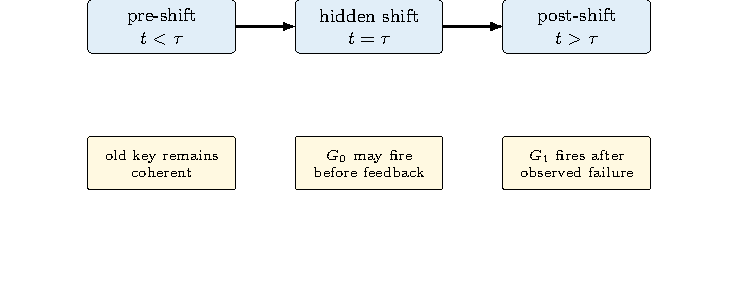
\includegraphics[width=0.74\textwidth,trim=14mm 14mm 14mm 0mm,clip]{fig_timeline.pdf}
\caption{The rule-shift timeline. Axon observes the trace on both sides of $\tau$ but receives no shift marker. The distinction between pre-shift coherence and post-shift wrongness is the source of the confident-wrong blind spot.}
\label{fig:timeline}
\end{figure}

\begin{figure}[H]
\centering
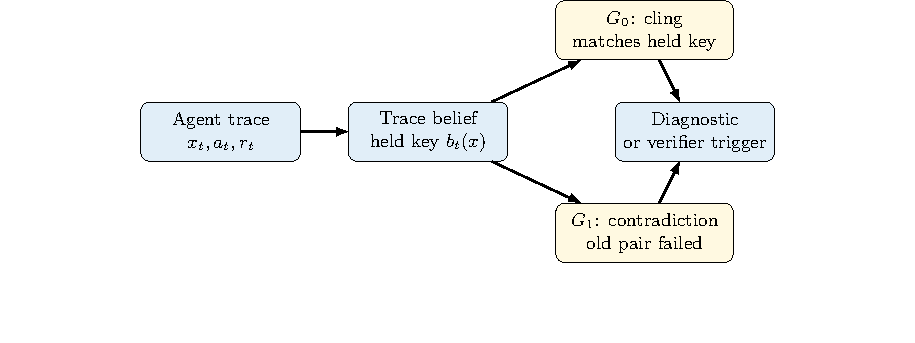
\includegraphics[width=0.74\textwidth,trim=23mm 12mm 23mm 0mm,clip]{fig_pipeline.pdf}
\caption{Axon's passive detector reads only the live trace. $G_0$ is anticipatory but can fire on unchanged items; $G_1$ is selective but waits for an observed contradiction. Both gates cost zero additional model calls.}
\label{fig:pipeline}
\end{figure}

\section{Notation and Evaluation Estimands}
\label{sec:notation}

Table~\ref{tab:notation} fixes the symbols used throughout the paper. We distinguish a
runtime quantity, which can be computed from $H_t$, from an evaluation quantity, which may
use $y_t$ after the episode has ended.

\begin{table}[!ht]
\centering\footnotesize
\setlength{\tabcolsep}{4pt}
\begin{tabular}{lll}
\toprule
Symbol & Meaning & Runtime visibility\\
\midrule
$\mathcal{X},\mathcal{A}$ & item and answer spaces & environment interface\\
$\theta^{\mathrm{pre}},\theta^{\mathrm{post}}$ & pre/post hidden rules & evaluation only\\
$\tau$ & registered shift time & evaluation only\\
$\mathcal{C},\rho$ & changed items and changed fraction & evaluation only\\
$x_t,a_t,y_t$ & item, model answer, correct answer & $y_t$ hidden\\
$r_t,z_t$ & reward and correctness indicator & $r_t$ visible\\
$H_t$ & observable history before step $t$ & visible\\
$b_t(x)$ & held key inferred from past answers & derived from $H_t$\\
$q_t$ & branch-vote agreement & visible\\
$s_m(t)$ & score from mechanism $m$ & derived from $H_t$\\
$\operatorname{AUROC}(s)$ & ranking wrong rows above right rows & evaluation\\
\bottomrule
\end{tabular}
\caption{Notation and information boundary. The evaluation-only columns are never passed to a detector during an episode.}
\label{tab:notation}
\end{table}

For a scalar score $s_t$, the primary estimand is

\begin{eqbox}
\begin{align*}
\operatorname{AUROC}(s)&=\Pr\bigl(s_t>s_u\mid z_t=0,\ z_u=1\bigr)\\
&\quad+\frac{1}{2}\Pr\bigl(s_t=s_u\mid z_t=0,\ z_u=1\bigr).
\end{align*}
\end{eqbox}

The score is useful when it ranks a wrong row above a right row, not merely when it has a high
mean. We therefore also report false-alarm rate and lead time. Let $T_f$ be the first firing
step of a detector in an episode and $T_w(x)$ the first failure step for a cue $x$ that later
fails. The cross-cue lead estimand is

\begin{eqbox}
\[
L=\frac{1}{|\mathcal{P}|}\sum_{(f,x)\in\mathcal{P}}
\bigl(T_w(x)-T_f\bigr),
\qquad
F=\frac{\#\{\text{unshifted correct rows fired}\}}
{\#\{\text{unshifted correct rows}\}},
\]
\end{eqbox}

where $\mathcal{P}$ contains comparable detector-warning/future-failure pairs. Positive $L$
means the warning precedes the later failure. $F$ is kept beside $L$ because an early detector
that fires on every correct unchanged row is not operationally useful.

\begin{definition}[Confidently-wrong row]
\label{def:confidentwrong}
A row at time $t$ is confidently wrong relative to a trace score $s$ when $z_t=0$ and
$s_t$ is at least as large as the score on a matched right row under the same evaluation
condition. In the paper's primary comparisons, this is operationalized by ranking wrong rows
above right rows with AUROC rather than by imposing an arbitrary score threshold.
\end{definition}

\paragraph{Remark (reaction bound for contradiction).}
For the gate $G_1$ defined above, the first firing time for an item $x$ cannot precede the
first observed zero-reward occurrence of the same $(x,a)$ pair. This follows directly from
the gate's information boundary: before such an observation enters $H_t$, the existential
condition in $G_1$ is false. The substantive question is empirical---how this reactive
constraint trades off against $G_0$'s earlier but less selective warnings.

\section{Related Work and Positioning}
\label{sec:related}

ReAct \citep{yao2023react} interleaves reasoning and acting, while Reflexion
\citep{shinn2023reflexion} adds verbal feedback across attempts. Semantic uncertainty and
self-consistency are useful when a model is unsure, but they do not directly represent the
possibility that a once-correct rule has become false. CLIN \citep{majumder2023clin} studies
continual adaptation, and WALL-E \citep{zhou2024walle} learns symbolic rules through a world
model. \axon{} differs in target and cost: it is a training-free diagnostic over a live trace,
with objective reward feedback and a registered mid-episode rule shift.

Axon's sequential signals are also related to classical concept-drift detection. Page's
CUSUM-style monitoring \citep{page1954}, drift detection method (DDM) \citep{gama2004}, and
ADWIN \citep{bifet2007} detect a change in an observed stream or error process, typically to
trigger model updating. \axon{} does not claim a new generic drift detector. It asks whether
a frozen agent's answer trace has become confidently wrong after a hidden rule shift, without
reading the hidden correctness label at runtime. In this framing, $G_1$ is a reward-grounded
contradiction signal and M3/M7 is a trace-only velocity-and-selection attempt; the measured
precision/earliness tradeoff and selector failure complement rather than replace classical
drift detectors.

\begin{table}[!ht]
\centering\footnotesize
\setlength{\tabcolsep}{3pt}
\begin{tabular}{p{24mm}p{30mm}p{39mm}p{15mm}}
\toprule
Method & Signal & Detects stale belief? & Model calls\\
\midrule
Self-consistency & vote agreement & No & $k$\\
Semantic entropy & answer distribution & No & $k$\\
Active probe & self-report question & No (falsified) & extra\\
\axon{} $G_0$ & trace belief consistency & Conditional & zero\\
\axon{} $G_1$ & observed contradiction & Conditional & zero\\
\bottomrule
\end{tabular}
\caption{Positioning of the evaluated signals. `No' means the signal does not detect the
confident-wrong regime in the tested setting; `Conditional' denotes a broad-shift condition
for $G_0$ and a reactive contradiction condition for $G_1$. The two gates are complementary,
not a solved selector.}
\label{tab:position}
\end{table}

\section{Detector Mechanisms}
\label{sec:mechanisms}

The final robust inventory contains four mechanisms. M1 is $G_0$ cling. M2 is $G_1$
contradiction. M3 is the raw rate of new contradictions in a short window. M7 is not a
second raw signal: it is the deterministic selector that consumes M3 and chooses between
$G_0$ and $G_1$. M5 is the parameter-free soft blend $G_0G_1$. M4 cross-item consensus, M6
agreement drop, and M8/M9 vote-shape selection were tested and dropped from the robust
inventory because they did not transfer consistently.
Later fact-stream runs show that some of these dropped mechanisms are environment-specific
signals; they are reported as such rather than called intrinsically useless.

Let $c_t=G_1(t)$ denote an observed contradiction and let $w$ be the short detector window.
The velocity and agreement-derived mechanisms are defined from the same trace:

\begin{eqbox}
\begin{align}
 d_t &= \sum_{i=t-w+1}^{t}c_i, &\text{contradiction density},\\
 v_t &= d_t-d_{t-1}, &\text{new-contradiction velocity},\\
 \bar q_t &= \frac{1}{w}\sum_{i=t-w}^{t-1}q_i, &\text{prior agreement},\\
 \Delta q_t &= \bar q_t-q_t, &\text{agreement drop}.
\end{align}
\end{eqbox}

M1 uses the held key directly, M2 uses $c_t$, and M3 uses $v_t$. M4 measures whether the
current answer agrees with the answers associated with other items in the current trace. M5
is a soft conjunction that avoids adding a learned weight. M6 uses $\Delta q_t$. M7 is the
registered velocity selector, with a fixed threshold $\lambda$:

\begin{eqbox}
\[
s_{M5}(t)=G_0(t)G_1(t),\qquad
s_{M7}(t)=
\begin{cases}
G_1(t),&v_t\geq\lambda,\\
G_0(t),&v_t<\lambda.
\end{cases}
\]
\end{eqbox}

For the vote-shape family, let $n_a(t)=\sum_j\ind{v_{t,j}=a}$. M8 is a split-vote score
that is high when two answers receive substantial support, and M9 uses that shape to choose
between the two gates:

\begin{eqbox}
\[
s_{M8}(t)=\frac{n_{(2)}(t)}{k},\qquad
s_{M9}(t)=\begin{cases}
G_1(t),&n_{(2)}(t)/k\geq\gamma,\\
G_0(t),&n_{(2)}(t)/k<\gamma,
\end{cases}
\]
\end{eqbox}

where $n_{(2)}$ is the second-largest vote count and $\gamma$ is fixed before evaluation.
These definitions make the negative result reproducible: the selector is a deterministic
function of the trace, not a post-hoc choice made after inspecting labels.

\begin{table}[!ht]
\centering\footnotesize
\setlength{\tabcolsep}{3pt}
\begin{tabular}{p{25mm}p{40mm}p{15mm}p{42mm}}
\toprule
Mechanism & Definition & Calls & Final role\\
\midrule
M1 / $G_0$ & answer matches held key & 0 & primary detector\\
M2 / $G_1$ & exact pair contradicted & 0 & partial-shift gate\\
M3 & raw contradiction velocity & 0 & selector input only\\
M7 & thresholded M3 chooses G0/G1 & 0 & non-dominant selector\\
M5 & $G_0G_1$ & 0 & non-dominant blend\\
M4, M6, M8/M9 & cross-item, agreement, vote shape & 0 & conditional signals\\
\bottomrule
\end{tabular}
\caption{The mechanism inventory after registered tests.}
\label{tab:mechanisms}
\end{table}

\begin{table}[!ht]
\centering\footnotesize
\setlength{\tabcolsep}{3pt}
\begin{tabular}{p{15mm}p{34mm}p{38mm}p{34mm}}
\toprule
Mechanism & Formal score & Information used & Interpretation\\
\midrule
M1 / $G_0$ & $\ind{a_t=b_t(x_t)}$ & prior answers & stale-key consistency\\
M2 / $G_1$ & $\ind{\exists i<t:r_i=0}$ & reward contradiction & confirmed failure\\
M3 & $v_t=d_t-d_{t-1}$ & recent contradictions & change velocity\\
M4 & cross-item agreement & other cue answers & shared-rule support\\
M5 & $G_0G_1$ & M1 and M2 & soft conjunction\\
M6 & $\Delta q_t=\bar q_t-q_t$ & branch agreement & confidence drop\\
M7 & thresholded $v_t$ selector & M1, M2, M3 & gate selection\\
M8 & $n_{(2)}(t)/k$ & vote histogram & bimodal uncertainty\\
M9 & thresholded M8 selector & M1, M2, M8 & vote-shape selection\\
\bottomrule
\end{tabular}
\caption{Formal mechanism definitions. All scores are trace functions; none receives the hidden post-shift label at runtime.}
\label{tab:formalmechanisms}
\end{table}

\begin{figure}[H]
\centering
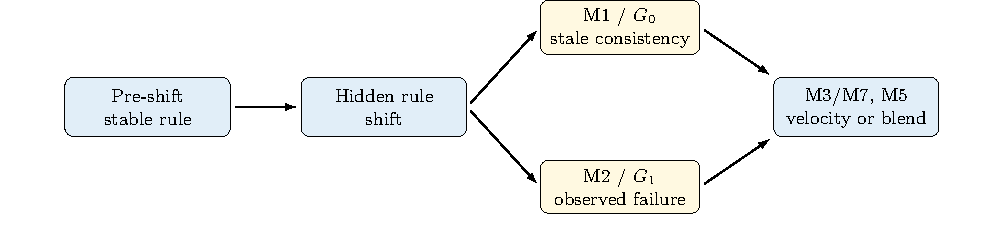
\includegraphics[width=0.70\textwidth]{fig_mechanisms.pdf}
\caption{Mechanism roles under rule shift. M3 is the raw contradiction-velocity statistic;
M7 is the selector derived from M3 that chooses between $G_0$ and $G_1$. The retained
inventory contains one anticipatory signal, one contradiction signal, and two attempted ways
to combine or select between them.}
\label{fig:mechanisms}
\end{figure}

\section{Evaluation Protocol}
\label{sec:protocol}

The primary metric is AUROC for ranking wrong rows above right rows. We report bootstrap 95\%
intervals, sample sizes, and every registered prediction outcome. The main environments are
RuleShift, a 12-entity fact-update stream, TruthfulQA content under a controlled modified
stream, TreeCut, and HotpotQA yes/no. Track A of the external benchmarks remains unmodified
and tests only the premise; Track B is always labelled as modified benchmark content under
rule shift.

The core RuleShift sweep uses three overlap levels: all items change, one item remains
unchanged, or two items remain unchanged. External sweep points use changed fractions 1.0,
0.7, and, for the fact stream, 0.3. No prediction band is widened after a result. Runs that
collapse a class or use an obviously easy distractor are excluded from headline claims and
recorded as setup failures.

The scale ladder uses `meta-llama/llama-3.2-3b-instruct`,
`meta-llama/llama-3.1-8b-instruct`, and `meta-llama/llama-3.3-70b-instruct`. These are
multiple checkpoints within the broad Llama family, not a clean intervention on parameter
count: the checkpoint generations differ. We therefore describe the comparison as
within-family transfer with a lower-capacity boundary, not as a causal scaling law.

For each condition, the confidence interval is obtained by resampling scored rows with
replacement and taking the 2.5th and 97.5th percentiles:

\begin{eqbox}
\[
\operatorname{CI}_{95}(s)=\left[Q_{0.025}
\left(\widehat{\operatorname{AUROC}}^{\,*}\right),
Q_{0.975}\left(\widehat{\operatorname{AUROC}}^{\,*}\right)\right].
\]
\end{eqbox}

The reported point estimate is computed once on the registered trace. Bootstrap intervals are
uncertainty summaries, not new tuning opportunities; thresholds and prediction bands remain
fixed after registration.

Table~\ref{tab:benchmarks} separates the diagnostic role of each condition from its transfer
role. The external Track B streams are controlled rule-shift transformations of benchmark
content; they are not claimed to be standard leaderboard evaluations.

\begin{table}[!ht]
\centering\footnotesize
\setlength{\tabcolsep}{3pt}
\begin{tabular}{p{24mm}p{25mm}p{28mm}p{18mm}p{16mm}}
\toprule
Condition & Hidden object & Shift design & Main scale & Rows\\
\midrule
RuleShift & key-to-answer rule & overlap 0/1/2 & 3B--70B & 240\\
FactStream & natural-language facts & $\rho=1.0,0.7,0.3$ & 3B/8B/70B & 600\\
TruthfulQA & modified fact answers & $\rho=1.0,0.7$ & 70B & 300\\
TreeCut & yes/no benchmark content & $\rho=0.7$ & 70B & 300\\
HotpotQA & yes/no benchmark content & $\rho=0.7$ & 70B & 300\\
\bottomrule
\end{tabular}
\caption{Evaluation suite. Unless explicitly pooled, $n$ is per listed condition: RuleShift
has 240 scored rows per overlap condition; FactStream has 600 per changed fraction and
backbone; each external benchmark has 300 per benchmark and shift fraction.}
\label{tab:benchmarks}
\end{table}

The measurement pipeline is intentionally label-separated. A generator produces the trace,
the detector scores the trace without labels, and a separate evaluator joins scores to the
hidden answer column only after the run. This is also where the project checks for the two
known setup confounds: a half-shift condition that accidentally leaves a class unchanged and
an easy distractor that inflates an apparent detector score.

\begin{figure}[H]
\centering
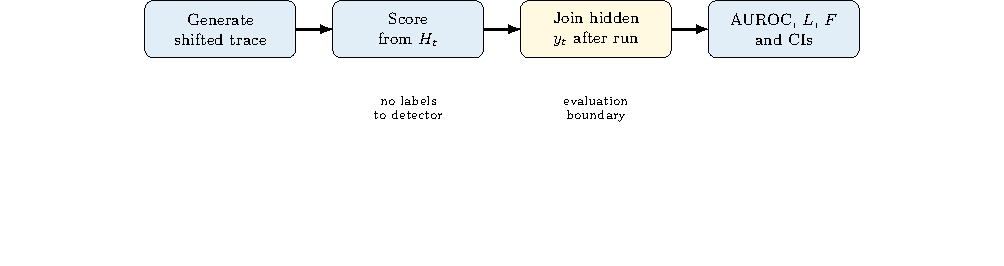
\includegraphics[width=0.82\textwidth,trim=23mm 23mm 23mm 0mm,clip]{fig_evaluation.pdf}
\caption{Evaluation separation. Detection uses the observable history; correctness labels are joined only in the offline scoring stage.}
\label{fig:evaluation}
\end{figure}

\section{The Confident-Wrong Blind Spot}
\label{sec:results}

On RuleShift at 70B, $G_0$ reaches AUROC 0.976 while self-consistency remains at 0.492. On
the 70B fact stream, $G_0$ reaches 0.761 at a full shift while uncertainty baselines remain
near chance. The direct curve is the simpler result: in RuleShift at 70B, accuracy falls from
1.000 to 0.571 while agreement moves only from 0.855 to 0.807. The model loses nearly half
its accuracy without a corresponding confidence collapse.

The 70B full-shift value is a stress-test condition, not a standalone discovery claim. In
that condition every previously rewarded key changes, so continued agreement with a stable
old key is partly aligned with wrongness by construction. The trace is not noiseless:
pre-shift branch agreement is 0.855, leaving 14.5\% disagreement, and $G_0$ fires on 95.1\%
of wrong rows and 0.0\% of right rows in the scored window. We therefore interpret the
0.976 result together with the partial-shift crossover, the fact-update stream, and the
external benchmark streams rather than treating it as evidence that a detector discovers an
arbitrary full-shift boundary.

\begin{table}[!ht]
\centering\small
\begin{tabular}{lrrr}
\toprule
Condition & $G_0$ & uncertainty agreement & semantic entropy\\
\midrule
RuleShift 70B, full shift & 0.976 & 0.492 & 0.492\\
Fact stream 70B, full shift & 0.761 & 0.472 & 0.474\\
TruthfulQA, full shift & 0.628 & 0.347 & 0.347\\
\bottomrule
\end{tabular}
\caption{The blind spot across environments. TruthfulQA is modified benchmark content in the stream condition.}
\label{tab:blindspot}
\end{table}

\begin{table}[!ht]
\centering\footnotesize
\setlength{\tabcolsep}{3pt}
\begin{tabular}{lrrrrr}
\toprule
Fresh $\rho=0.7$ condition & $G_0$ & $G_1$ & M5 & M7 & M9\\
\midrule
TruthfulQA & \aucci{.517}{.490}{.546} & \aucci{.610}{.565}{.654} & \aucci{.620}{.578}{.660} & \aucci{.568}{.510}{.626} & \aucci{.513}{.490}{.539}\\
TreeCut & \aucci{.506}{.479}{.534} & \aucci{.644}{.610}{.678} & \aucci{.641}{.607}{.676} & \aucci{.566}{.506}{.626} & \aucci{.506}{.479}{.534}\\
HotpotQA & \aucci{.520}{.502}{.542} & \aucci{.639}{.603}{.676} & \aucci{.653}{.621}{.686} & \aucci{.585}{.526}{.644} & \aucci{.516}{.499}{.535}\\
\bottomrule
\end{tabular}
\caption{Fresh external comparison at a 70\% changed fraction, $n=300$ per condition.
Cells show AUROC [95\% bootstrap CI]. Partial shifts reverse the broad-shift ordering:
contradiction and soft-blend scores exceed cling; overlapping intervals should not be read as
evidence of a resolved difference between those two scores.}
\label{tab:external}
\end{table}

The fact stream also exposes a deployment boundary. At 70B, $G_0$ scores 0.387 on items
seen zero or one time before the shift, 0.654 on items seen two to four times, and 0.866 on
items seen at least five times. A gate cannot read a belief that the agent has not formed.

\section{Cross-Scale and Cross-Environment Results}
\label{sec:generalization}

The detector is not a RuleShift-only case study, but the scale boundary is real. On the fact
stream under a full shift, $G_0$ scores 0.498 at 3B, 0.786 at 8B, and 0.761 at 70B. The
3B model is too weak to provide a stable belief in this larger, unevenly sampled item space;
the 8B and 70B rows reproduce the detector result.

The shift-fraction crossover is more stable than any single point. At 70B on the fact stream,
$G_0$ scores 0.761, 0.466, and 0.367 as the changed fraction moves from 1.0 to 0.7 to 0.3.
$G_1$ scores 0.505, 0.636, and 0.665. The same direction appears on the three independent
external benchmark streams at the 0.7 point. Broad shifts make stale consistency informative;
partial shifts make that same consistency correct on too many unchanged items.

\begin{table}[!ht]
\centering\footnotesize
\setlength{\tabcolsep}{4pt}
\begin{tabular}{lrrrr}
\toprule
FactStream backbone & $G_0$ & $G_1$ & M7 & M5\\
\midrule
Llama 3.2 3B & \aucci{.498}{.453}{.546} & \aucci{.420}{.385}{.458} & \aucci{.480}{.437}{.526} & \aucci{.433}{.387}{.482}\\
Llama 3.1 8B & \aucci{.786}{.736}{.833} & \aucci{.602}{.535}{.664} & \aucci{.739}{.684}{.790} & \aucci{.686}{.639}{.728}\\
Llama 3.3 70B & \aucci{.761}{.725}{.794} & \aucci{.505}{.448}{.564} & \aucci{.665}{.616}{.710} & \aucci{.665}{.645}{.685}\\
\bottomrule
\end{tabular}
\caption{Cross-scale AUROC [95\% bootstrap CI] on the full-shift fact stream, $n=600$ per
backbone row. The detector requires a sufficiently stable trace belief; scale alone is not a
guarantee because the 70B and 8B rows are not identical.}
\label{tab:scale}
\end{table}

\section{Early Warning and Its Cost}
\label{sec:lead}

Because a gate is evaluated on the current answer, a per-item lead would be zero by
construction. We therefore use cross-item transfer: the first firing step on any item is
compared with the first failure step of each item that later fails. This measures whether an
early warning on one item precedes failures on others.

\begin{table}[!ht]
\centering\small
\begin{tabular}{lrrrr}
\toprule
Condition & $G_0$ lead & $G_0$ FA ($n$) & $G_1$ lead & $G_1$ FA ($n$)\\
\midrule
RuleShift 3B full & \leadci{+1.24}{.78}{1.70} & .000 (7) & \leadci{-.45}{-.95}{.10} & .143 (7)\\
RuleShift 8B full & \leadci{+.91}{.45}{1.37} & .167 (6) & \leadci{-.25}{-.71}{.24} & .167 (6)\\
RuleShift 70B full & \leadci{+1.65}{1.24}{2.07} & .000 (4) & \leadci{-1.27}{-1.92}{-.59} & .000 (4)\\
Fact stream 70B full & \leadci{+5.76}{5.07}{6.45} & .026 (116) & \leadci{+2.57}{1.78}{3.35} & .000 (116)\\
TruthfulQA full & \leadci{+3.62}{3.21}{4.02} & .072 (166) & \leadci{+.82}{.31}{1.31} & .096 (166)\\
TreeCut 70\% shift & \leadci{+3.73}{3.28}{4.23} & .310 (226) & \leadci{-1.16}{-1.71}{-.60} & .000 (226)\\
HotpotQA 70\% shift & \leadci{+3.74}{3.26}{4.22} & .323 (226) & \leadci{-1.17}{-1.73}{-.59} & .004 (226)\\
\bottomrule
\end{tabular}
\caption{Cross-cue mean lead [95\% bootstrap CI]. FA is the false-alarm rate; its parenthetic
denominator is the number of unfailing cues. False alarms are mandatory context for
interpreting earliness.}
\label{tab:lead}
\end{table}

The result is a frontier, not a single winner. $G_0$ is early and can be used as a cheap
trigger for a verifier, but it cries wolf under partial shifts. $G_1$ is later and selective.
The fact stream and TruthfulQA results also show that a contradiction gate can warn about
later failures in a larger item space, even though its first contradiction is necessarily
reactive.

\begin{figure}[H]
\centering
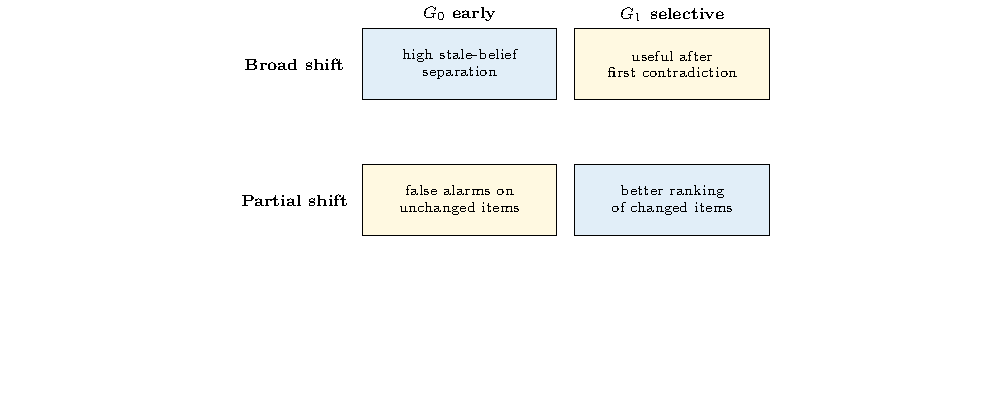
\includegraphics[width=0.72\textwidth,trim=39mm 28mm 39mm 0.5mm,clip]{fig_frontier.pdf}
\caption{The measured detector frontier. Shift breadth changes which gate is useful, which is why the tested runtime selectors do not yield a robust universal choice.}
\label{fig:frontier}
\end{figure}

\section{Mechanism Ablation and Failed Self-Report}
\label{sec:ablation}

The four-mechanism ablation confirms the complementarity of the gates. On RuleShift, M1/G0
scores 0.776, 0.515, and 0.364 as overlap increases. M2/G1 scores 0.592, 0.748, and
0.746. M3/M7 scores 0.721, 0.620, and 0.616, while M5 scores 0.634, 0.682, and 0.637.
Neither combination dominates selecting the correct gate with knowledge of the condition.

\begin{table}[!ht]
\centering\footnotesize
\setlength{\tabcolsep}{4pt}
\begin{tabular}{lrrrr}
\toprule
Unchanged cues & M1 / $G_0$ & M2 / $G_1$ & M7 selector & M5 blend\\
\midrule
0 of 12 & \aucci{.776}{.721}{.827} & \aucci{.592}{.517}{.668} & \aucci{.721}{.664}{.774} & \aucci{.634}{.578}{.686}\\
1 of 12 & \aucci{.515}{.452}{.577} & \aucci{.748}{.698}{.796} & \aucci{.620}{.560}{.682} & \aucci{.682}{.638}{.728}\\
2 of 12 & \aucci{.364}{.302}{.428} & \aucci{.746}{.691}{.798} & \aucci{.616}{.552}{.678} & \aucci{.637}{.591}{.687}\\
\bottomrule
\end{tabular}
\caption{Registered RuleShift ablation, AUROC [95\% bootstrap CI], $n=240$ per overlap row.
Broad shifts favor cling; partial shifts favor contradiction. The selector does not identify
this condition robustly from the trace alone.}
\label{tab:ablation}
\end{table}

The ablation can also be read as a conditional decision problem. If the shift breadth $\rho$
were available, an oracle selector could choose

\begin{eqbox}
\[
s_{\mathrm{oracle}}(t;\rho)=
\begin{cases}
s_{G_0}(t),&\rho\text{ is broad},\\
s_{G_1}(t),&\rho\text{ is partial}.
\end{cases}
\]
\end{eqbox}

Axon's runtime problem is that $\rho$ is exactly the quantity the model and detector do not
observe. The table therefore measures a genuine information gap rather than an unfinished
hyperparameter search.

The active probe asks the model whether its old rule would still predict the observation. Once
the earlier oracle confound was removed and the probe used the model's inferred belief, the
probe was at chance across all overlap levels. The bare trace gate matched or beat it. The
negative result is important: a frozen model cannot reliably self-report that its own rule
belief has gone stale, even when it can continue producing a confident answer.

\section{The Detectability Limit}
\label{sec:limit}

The central limit is not simply that small shifts are hard. The gate can become confidently
backwards. On RuleShift, $G_0$ AUROC decays from 0.775 at a full shift to 0.515 with one
unchanged cue and 0.364 with two unchanged cues. On external benchmark content at 70\% changed,
$G_0$ sits near chance while $G_1$ is between 0.60 and 0.64 on all three benchmarks.

Twelve selector variants were tested, including density thresholds, confirmed density,
velocity, cross-item consensus, agreement drop, vote shape, and blends. None robustly selected
the right gate across conditions. New fact-stream runs show that M4, M6, and M8 can be
informative in particular environments, but their behavior changes with scale and shift
fraction. The honest conclusion is therefore not that every signal fails everywhere; it is
that no tested runtime rule is robust enough to replace the measured tradeoff.

\section{Limitations and Future Work}
\label{sec:limitations}

First, the detector is only as good as the belief it reads. Rare items and the 3B fact-stream
condition show the lower boundary. Second, the active probe result is a negative result for
the tested self-report design, not a theorem that no future model can answer such a question.
Third, the shift fraction is not directly observable early enough for the tested selectors to
choose reliably. Fourth, external Track B conditions are controlled modified streams and must
not be described as unmodified benchmark evaluations. Finally, M4, M6, and M8 show useful
environment-specific behavior, so future work should study conditional activation rather than
add more fixed selectors.

\paragraph{Companion-paper application.}
\axon{} is the diagnostic companion to \probe{}, which uses explicit belief revision as an
intervention. These are imported PROBE results rather than Axon experiments: on the
single-factor I3 rule shift, baseline and PROBE post-shift accuracies are 0.390 and 0.393
over 50 episodes, an honest tie; on the mixed/multi-factor I6 shift, they are 0.509 and 0.750
over 40 episodes. The connection is therefore conditional: Axon identifies stale confidence,
while PROBE's structured revision helps most where its extra machinery changes adaptation.

\section{Conclusion}
\label{sec:conclusion}

Language models can be confidently wrong because a rule that was once correct remains coherent
after the world changes. \axon{} detects this stale-confidence regime with a zero-call gate
over the agent's own trace. It generalizes across scales and environments when a belief is
formed, fires early with a measurable false-alarm tradeoff, and exposes why ordinary uncertainty
signals fail. The remaining boundary is equally important: no tested runtime selector robustly
knows whether a shift is broad enough for clinging to be dangerous. That honest limit defines
the next research problem and gives \probe{} a precise diagnostic trigger.

\section*{Data and Code Availability}

The Axon workspace contains the trace-generation scripts, registered predictions, raw traces,
scoring scripts, and the full chronological research log. The PROBE cross-link uses existing
versioned PROBE traces and is labeled separately from Axon-generated experiments.

\appendix
\section{Glossary}
\begin{table}[!ht]
\centering\small
\begin{tabular}{p{0.28\textwidth}p{0.64\textwidth}}
\toprule
Term & Meaning\\
\midrule
confidently-wrong row & a wrong answer ranked as highly suspicious as or more suspicious than a right row under the same condition\\
rule shift & a change from $\theta^{\mathrm{pre}}$ to $\theta^{\mathrm{post}}$ during an episode\\
changed fraction $\rho$ & proportion of items whose rewarded answer changes\\
trace belief & the key inferred from an agent's previous answers for an item\\
cling gate $G_0$ & zero-call detector for continuing to answer with the held key\\
contradiction gate $G_1$ & zero-call detector activated by an earlier zero-reward pair\\
velocity $v_t$ & change in recent contradiction density\\
soft blend M5 & the parameter-free conjunction $G_0G_1$\\
runtime selector & a trace-only rule that chooses between detector gates\\
cross-cue lead & warning time on one item before a later failure on another\\
Track B & controlled modified benchmark content under a declared rule shift\\
frozen backbone & the language model used without weight updates\\
\bottomrule
\end{tabular}
\caption{Glossary of Axon terms (appendix).}
\label{tab:glossary}
\end{table}

\begingroup
\small
\setlength{\bibsep}{3pt}
\bibliography{references}
\endgroup

\end{document}
